 \section{Das Materialsystem Zinkoxid (ZnO)}
\label{ZnOMat}
Zinkoxid (ZnO) ist ein $\text{II}^\text{b}$-VI Verbindungshalbleiter mit einer direkten Bandlücke von  $\text{E}_\text{g}= (\text{3.37} \pm \text{0.01})$ eV bei Raumtemperatur am $\Upgamma$-Punkt \cite{Klingshirn.2010}. Durch das \mbox{Kristallfeld} und die Spin-Bahn-Wechselwirkung wird das Valenzband (kurz \textit{VB}) in drei \mbox{Subbänder} aufgespalten (A, B und C, bzw. \textit{heavy hole (HH)}, \textit{light hole (LH)} und \textit{split off (SO)}) – die Energiedifferenzen betragen $\Updelta \text{E}_\text{AB}= \text{4.9}$ meV und $\Updelta \text{E}_\text{BC}= \text{43.7}$ meV \cite{Klingshirn.2010}.
Hierbei wird dem B-Valenzband die Symmetrie $\Upgamma_\text{9}$ zugeordnet, den anderen beiden \mbox{Valenzbändern} A und B sowie dem Leitungsband die Symmetrie $\Upgamma_\text{7}$. Dies führt dazu, dass einige \mbox{Dipolübergänge} stark unterdrückt sind, je nachdem ob der Vektor des \mbox{elektrischen} \mbox{Feldes} $\vec{\textbf{E}}$ parallel oder vertikal zur c-Achse des Kristalls ausgerichtet ist. Die \mbox{verschiedenen} Übergange sind in \autoref{spinueb} zusammengefasst. \\
%Dies ist eine ungewöhnliche Anordnung, verglichen mit den meisten anderen Halbleitern, welche die $\Upgamma_\text{9}$-Symmetrie im obersten Valenzband zeigen, und wurde von Hopfield (1960) beschrieben \cite{Hopfield.1960}, ist aber seitdem umstritten \cite{Park.1966}, denn für beide Anordnungen gibt es Argumente, die hier im Rahmen dieser Arbeit aber nicht weiter erläutert werden sollen. Für den Übergang $\Upgamma_\text{9}[\text{B}]\longrightarrow \Upgamma_\text{7}$ gilt die Auswahlregel, dass der elektrische Feldvektor des Lichts orthogonal auf der c-Achse des Kristallgitters stehen muss ($\vec{\textbf{E}} \bot \vec{\textbf{c}}$), für die Übergänge  $\Upgamma_\text{7}[\text{A,C}] \longrightarrow \Upgamma_\text{7}$ kann dieser zusätzlich auch parallel ausgerichtet sein (sowohl $\vec{\textbf{E}} \bot \vec{\textbf{c}}$ als auch $\vec{\textbf{E}} \| \vec{\textbf{c}}$ möglich)\cite{Thomas.1962}.\\
Zinkoxid kristallisiert unter Normalbedingungen bevorzugt in der hexagonalen Wurzit-Struktur, schematisch dargestellt in \autoref{ZnO} a), mit den Gitterkonstanten \mbox{$\text{a}= \text{b} = \text{3.25} \AA$} und $\text{c} = \text{5.20} \AA$ \cite{Klingshirn.2010}. Jedes Zinkatom ist dabei von vier Sauerstoffatomen \mbox{umgeben} und andersherum. Die tetraedale Bindungsstruktur wird von $\text{sp}^\text{3}$-Hybridorbitalen \mbox{geformt} und besitzt einen kovalenten Bindungscharakter, wobei die komplett \mbox{gefüllten} \mbox{2p-Orbitale} des Sauerstoffs (O) das Valenzband, die leeren 4s-Orbitale des Zink (Zn) das Leitungsband formen. Durch den hohen Elektronegativitätsunterschied  von \mbox{Sauerstoff} und Zink ($\Updelta\upchi\approx \text{1.8}$) hat die Bindung einen hohen ionischen Bindungsanteil. Die Stärke dieser ionischen Bindung beträgt 0.62 auf der Phillips-Skala \cite{Ivanov.1981} und liegt somit auf der Grenze zwischen ionischer und kovalenter Bindung.  Zinkoxid ist ein optisch anisotropes Medium mit den Brechungsindizes $\text{n}_\text{o}= \text{2.382}$  und $\text{n}_\text{ao}= \text{2.358}$ in der Nähe der Energie der Bandlücke für $\uplambda= \text{382}$ nm ($\text{E}_\text{Photon}= \text{3.246}$ eV) bei 4K \cite{Park.1968}. Die Dispersion bei $\uplambda=\text{390 nm}$ beträgt $\text{d} \text{n}/\text{d} \uplambda\approx \text{-4.30} \upmu \text{m}^\text{-1}$ \cite{Bond.1965}.
\begin{table}[h]
\centering
\begin{footnotesize}
\begin{tabular}{llll}
Exzitonenzustand & Dipolübergang & Spin-Flip & Übergangswahrscheinlichkeit\\
\toprule
A $\Upgamma_\text{1}$ & erlaubt (für $\vec{\textbf{E}} \| \vec{\textbf{c}}$) & ja & klein\\
A $\Upgamma_\text{2}$ & verboten & ja & sehr klein\\
A $\Upgamma_\text{5}$ & erlaubt (für $\vec{\textbf{E}} \bot \vec{\textbf{c}}$) & nein & groß\\
\midrule
B $\Upgamma_\text{6}$ & verboten & ja & sehr klein\\
B $\Upgamma_\text{5}$ & erlaubt (für $\vec{\textbf{E}} \bot \vec{\textbf{c}}$) & nein & groß\\
\midrule
C $\Upgamma_\text{1}$ & erlaubt (für $\vec{\textbf{E}} \| \vec{\textbf{c}}$) & nein & groß\\
C $\Upgamma_\text{2}$ & verboten & ja & sehr klein\\
C $\Upgamma_\text{5}$ & erlaubt (für $\vec{\textbf{E}} \bot \vec{\textbf{c}}$) & ja & klein\\
\end{tabular}
\end{footnotesize}
\caption[Auswahlregeln der Anregung für Exzitonen]{Die Auswahlregeln für Übergänge der A-, B- und C-Exzitonen von ZnO für $\text{n}_\text{B}=\text{1}$ ins Leitungsband mit ihren relativen Häufigkeiten (aus \cite{Klingshirn.2010})}
\label{spinueb}
\end{table}
\begin{figure}[h]
\centering
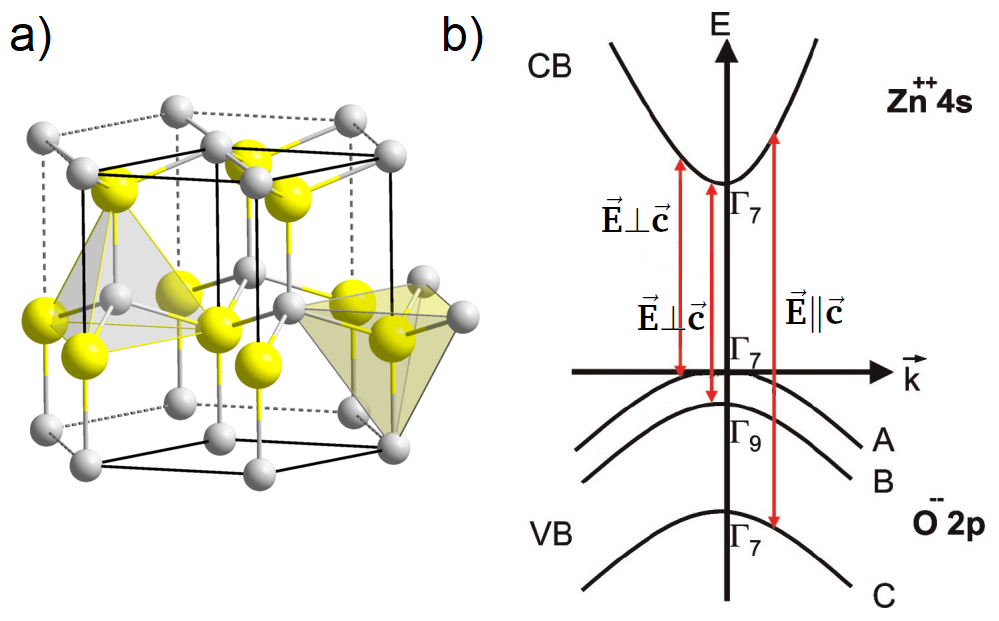
\includegraphics[width=.8\textwidth]{Bilder/ZnO_Str_BG}
\caption[ZnO Kristall- und Bandstruktur]{Darstellung der a) hexagonalen Wurzit-Struktur von ZnO mit Zn (gelb) und O (grau) (aus \cite{wurzite}) sowie der b) Bandstruktur von ZnO um den $\Upgamma$-Punkt mit den verschiedenen Subbändern nach (\cite{Klingshirn.2010}).}
\label{ZnO}
\end{figure}
\section{Lumineszenz in II$^b$-VI Halbleitern}
\label{ExAn}
Dieser Abschnitt soll eine Übersicht über die wichtigsten exzitonischen Prozesse im Material geben. Diese sind notwendig, um ein Verständnis für das optische Verhalten von Halbleitern unter Anregung zu schaffen und ihre Emissionseigenschaften zu verstehen.
\subsection{Exzitonen}
Trifft ein Photon mit einer Energie größer oder gleich der Bandlücke zwischen Valenz- und Leitungsband $\text{E}_\text{Photon} \geq \text{E}_\text{g}$ auf ein Medium, so kann es absorbiert werden. Im Falle der Absorption wird ein Elektron aus dem Valenzband in das Leitungsband angehoben, zurück bleibt eine geladene Fehlstelle (\textit{Loch}). Um die Energie zu minimieren relaxieren beide Ladungen materialabhängig im Piko- bis Femtosekundenbereich an die jeweilige Bandkante (Unterkante des Leitung- bzw. Oberkante des Valenzbandes). Die überschüssige Energie wird in Form von Gitterschwingungen (\textit{Phononen}) an den Festkörper abgegeben. Ein solches Elektron-Loch-Paar kann in seiner Beschreibung als Quasiteilchen betrachtet werden, man spricht von einem \textit{Exziton}. Dieses Exziton wird durch die Coulombkraft zwischen Elektron und Loch räumlich zusammengehalten und kann sich im Falle des \textit{freien Exzitons} (\textit{FX}) im Kristall bewegen. Ähnlich dem Wasserstoffatom kann man auch für das Exziton einen Bohr'schen Radius $\text{a}_\text{b}$ definieren, der die Ausdehnung des Exzitons beschreibt:
\begin{equation}
&a_b=\dfrac{\epsilon\hslash^2}{e^2 \mu_{FX}} &\mu_{FX}=\frac{(m_e^{\ast} \cdot m_h^{\ast})}{(m_e^{\ast} + m_h^{\ast})}=\frac{(m_e^{\ast} \cdot m_h^{\ast})}{M}\text{ ,}
\end{equation}
mit der Permittivität $\upepsilon$ und  der reduzierten Masse des Exzitons $\upmu_\text{FX}$.\\\\
Die Näherung der effektiven Masse besitzt jedoch nur dann Gültigkeit, wenn die \mbox{Ausdehnungen} des Exzitons größer als die Elementarzelle des Materialsystems \mbox{ist \cite{Klingshirn.2007}}.
Für ZnO ($\text{a}_\text{b}= \text{1.8}$ nm \cite{Haranath.2009} gegen $\text{c}= \text{0.52}$ nm) ist dies erfüllt. Solch schwach \mbox{gebundene} Exzitonen werden auch als \textit{Mott-Wannier-Exzitonen} bezeichnet.
Die Energie des freien Exzitons beträgt
\begin{equation}
E_X(\vec{\textit{\textbf{k}}},n_B)= E_g - R_y\frac{\mu_{FX}}{m_0\epsilon^2} \frac{1}{n_B^2} +\frac{\hslash^2\vec{\textit{\textbf{k}}}^2}{2M} \textit{ ,}
\label{EX}
\end{equation}
mit der Rydbergkonstante $\text{R}_\text{y}$, der Ruhemasse des Elektrons $\text{m}_\text{0}$, der Hauptquantenzahl des Exzitons $\text{n}_\text{B}= 1, 2, ..$ sowie dem Wellenvektor des Exzitons $\vec{\textbf{k}}= \vec{\textbf{k$_\text{e}$}}+\vec{\textbf{k$_\text{h}$}}$. Hierbei wird der zweite Term oft als Exziton-Bindungsenergie bezeichnet, der dritte Term enthält die kinetische Energie des Exzitons. Die Ausprägung der Bindungsenergie ist dabei \mbox{maßgeblich} von der Abschirmung durch die Valenzelektronen des \mbox{Materialsystems} bestimmt. Je lokalisierter diese sind, desto geringer ist die Abschrimung \cite{Dvorak.2013}. Für ZnO ergeben sich  Bindungsenergien zu $\text{E}_\text{X,ZnO}=$ 49...63 meV \cite{Mang.1995} bei $\text{n}_\text{B}= 1$ für die drei \mbox{Subbänder} A, B und C; die Lebensdauer liegt typischerweise im Bereich von einigen \mbox{hundert Pikosekunden \cite{Zhang.2007}}. Die Exzitonen des Materialsystems sind bei \mbox{Raumtemperatur} stabil, da die Bindungsenergien höher sind als die thermische Energie ($\text{k}_\text{b}\text{T} \approx 25$ meV). Für thermische Energien größer der Bindungsenergie der Exzitonen dissoziieren diese.\\
Bei den meisten Halbleiter, so auch in ZnO, kann die exzitonische Anregung des \mbox{Kristalls} nicht unabhängig vom Lichtfeld betrachtet werden, da hier eine starke \mbox{Kopplung} \mbox{auftritt}. Ein Photon bringt in den Kristall eine Polarisation in Form eines Exzitons ein. Das \mbox{Exziton} rekombiniert und emittiert ein Photon usw. Dieses Quasiteilchen aus Exziton und Photon wird als \textit{Exziton-Polariton} bezeichnet \cite{Hopfield.1958}. Die dazugehörige \mbox{Dispersion} ergibt sich aus der exakten Diagonalisierung des Hamilton-Operators für das gekoppelte System aus Exziton und Photon. Die Dispersion wird dargestellt in \autoref{PolScat}. Hierbei stellt der obere Ast (engl. \textit{upper polariton branch}, kurz \textit{UPB}) die Dispersion der longitudinalen exzitonischen Polarisation (die nicht mit dem \mbox{Lichtfeld} koppelt), der untere Ast (eng. \textit{lower polariton branch}, kurz \textit{LPB}) die \mbox{transversale} \mbox{exzitonische} \mbox{Polarisation} dar. Oberhalb der Exziton-Resonanz $\text{E}_\text{0}$ erfährt das \mbox{Lichtfeld} die Hintergrunds-Dielektrizitätskonstante $\upvarepsilon _\text{b}=\upvarepsilon (\infty)$, für Energien darunter die \mbox{statische} Dielektrizitätskonstante $\upvarepsilon _\text{s}=\upvarepsilon (\text{0})$. Somit folgt im UPB die Dispersion für \mbox{kleine} \mbox{Werte} $\vec{\textbf{k}}$ zunächst der exzitonischen Dispersion und nähert sich für größere Werte der \mbox{photonischen} Dispersion mit der Steigung $\text{c}/\sqrt{\upvarepsilon _\text{b}}$ an. Im LPB ist es genau \mbox{andersherum} mit der entsprechenden Steigung der photonischen Dispersion $\text{c}/\sqrt{\upvarepsilon _\text{s}}$. Polaritonen mit Energien sehr viel größer $\text{E}_\text{L}$, respektive Energien sehr viel kleiner $\text{E}_\text{0}$, besitzen folglich einen photonischen Charakter. Anregungen, wie sie in dieser Arbeit Anwendung finden, geschehen im UPB und können über akustische oder optische Phononenzweige ins LPB relaxieren \cite{Klingshirn.2007}.\\
\begin{figure}[htb]
\centering
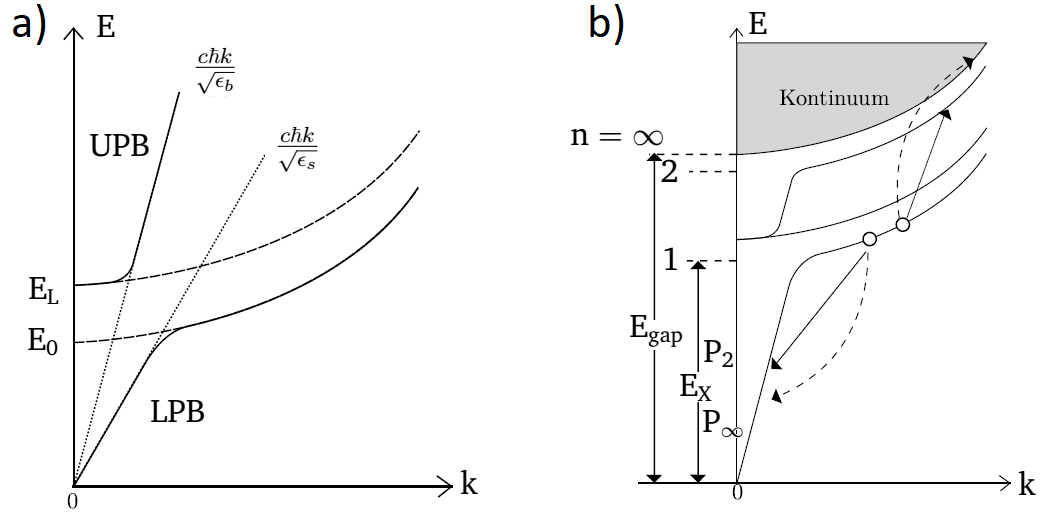
\includegraphics[width=1\textwidth]{Bilder/PolScat}
\caption[Polaritonendispersion und inelastische X-X-Streuung]{Schematische Darstellung der a) Dispersion des Exziton-Polaritons im UPB und LPB. Ebenfalls eingezeichnet, die Dispersion für Exzitonen (gestrichelt) und Photonen (gepunktet), sowie der b) inelastischen X-X-Streuung mit P$_\text{2}$($\longrightarrow$) und P$_\infty$ ($\dashrightarrow$) (beide aus \cite{Richters.Diss}).}
\label{PolScat}
\end{figure}
\subsection{Mehr-Exziton-Prozesse}
Treffen nun ausreichend viele Photonen passender Energie pro Zeit und Volumen- element auf ein Material, so erhöht sich die Zahl der erzeugten Exzitonen, so kann die Wechselwirkung zwischen den einzelnen Exzitonen nicht mehr vernachlässigt \mbox{werden} (s. \autoref{regimes}) – man spricht vom Bereich mittlerer Anregungsdichte. Es kommt \mbox{vermehrt} zu elastischen und inelastischen Streuprozessen von Exzitonen an \mbox{Exzitonen} (\textit{X-X-Streuung}) und an Ladungsträgern \textit{(X-e-} bzw. \textit{X-h-Streuung}). Es können sich Bi-Exzitonen (\textit{X$_\text{2}$}), bestehend aus zwei Exzitonen analog zum H$_\text{2}$-Molekül sowie höhere Anregungszustände ausbilden \cite{Corfdir.2011}. Die elastische Streuung der Exzitonen an einander sorgt hierbei für eine Erweiterung der Resonanz der Exzitonen, reduziert aber \mbox{gleichsam} ihre Lebensdauer. Bei inelastischer Streuung wird ein Exziton in einen \mbox{höheren} exzitonischen Zustand gehoben, während das andere auf den photonischen Ast der Exziton-Polaritondispersion gestreut wird. Die hierbei entstehende P-Bande wird je nach erreichtem Endanregungszustand des in den höheren Zustand gestreuten Exzitons mit P$_\text{2}$, P$_\text{3}$, ..., P$_\infty$ bezeichnet (s. \autoref{PolScat}). Das so gestreute Exziton relaxiert über Phononen-Streuung wieder zurück in den Grundzustand \cite{Klingshirn.1975}.
Da an diesem Streuprozess zwei Exzitonen teilnehmen, steigt die Intensität der P-Bande quadratisch mit der Anregungsdichte an \cite{Priller.2004}. Die strahlende Rekombination für Biexzitonen erzeugt die sogenannte M-Bande, die für ZnO ca. 12..20 meV unterhalb der Energie des freien Exzitons angesiedelt ist. Hierbei findet ein Zwei-Polariton-Zerfall statt, bei dem zumeist ein exzitonähnliches und ein photonähnliches Polariton entsteht, die Entstehung zweier photonähnlicher Polaritonen ist jedoch auch möglich \cite{Hvam.1983}. 
\begin{figure}[htb]
\centering
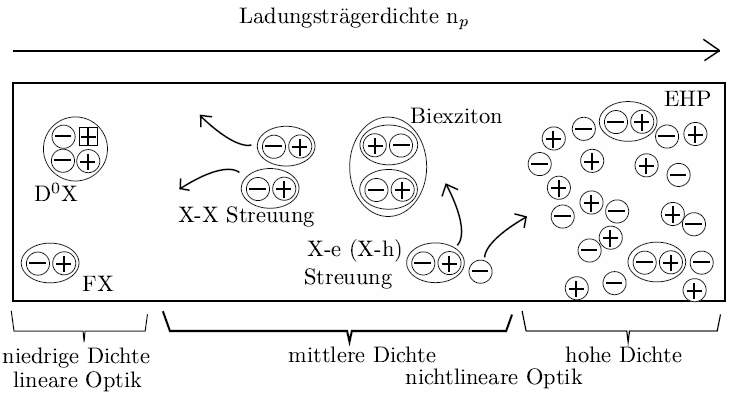
\includegraphics[width=0.6\textwidth]{Bilder/regimes}
\caption[Übersicht Exzitonen unter hohen Anregungsdichten]{Schematische Übersicht möglicher Quasiteilchen und deren Wechselwirkung unter verschiedenen Anregungsdichten (aus \cite{Richters.Diss}).}
\label{regimes}
\end{figure}
\subsection{Elektron-Loch-Plasma}
\label{EHP}
Bei noch höheren Anregungsdichten geht das Gesamtsystem in das so genannte Elektron-Loch-Plasma (engl. \textit{electron-hole-plasma}, kurz \textit{EHP}) über. Das EHP bezeichnet das Regime hoher Anregungsdichten und beginnt, sobald der mittlere Abstand der Exzitonen voneinander in etwa ihrem Bohr-Radius a$_\text{B}$ entspricht. Daraus folgt für die kritische Anregungsdichte n$_\text{p}^\text{c}\approx$ a$_\text{B}^\text{-3}$ \cite{Klingshirn.2007}. Ab dieser Anregungsdichte ist die Abschirmung der Teilchen untereinander so groß, dass man nicht mehr unterscheiden kann, welches Elektron an welches Loch gebunden ist. Die Definiertheit der Exzitonen verschwimmt, so dass nicht mehr von einem Quasipartikel, sondern vielmehr noch von einem Plasma gesprochen werden kann (s. \autoref{regimes}). Durch die starke Abschirmung der Coulombwechselwirkung kommt es zu einer Verminderung der Bandlückenenergie – man spricht von der sogenannten \textit{Bandlückenrenormierung}. Diese Renormierung folgt aus dem Pauli-Prinzip, das verbietet, dass sich zwei Elektronen gleichen Spins im Phasenraum einer Elementarzelle aufhalten. Es ist somit wahrscheinlicher, dass sich in unmittelbarer Nähe des Elektrons ein Loch aufhält als ein zweites Elektron. Somit überwiegen die anziehenden Coulombkräfte über die abstoßenden, sodass die Bandlücke hierdurch verringert wird \cite{Klingshirn.2007}. Im EHP sind sowohl Valenz- als auch Leitungsband bis zu den Quasiferminiveaus E$_\text{F}^\text{e}$ und E$_\text{F}^\text{h}$ gefüllt. Die Energiedifferenz dieser beiden Niveaus wird als chemisches Potential $\upmu$ bezeichnet.
\begin{figure}[h]
\centering
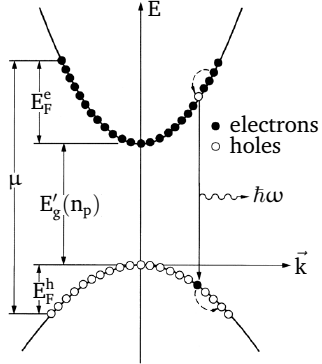
\includegraphics[width=0.5\textwidth]{Bilder/ehp}
\caption[Besetzung im EHP]{Schematische Darstellung der Besetzung in einem EHP mit Rekombinationsprozess nach \cite{Klingshirn.2007}.}
\label{Besetzung im EHP}
\end{figure}
\newpage
\noindent
Bei steigenden Anregungsdichten laufen die Quasiferminiveaus auseinander, so dass die spektrale Breite des Spektrums bei strahlender Rekombination
\begin{equation}
&\Delta E=\mu -E_g \qquad \qquad \qquad \text{mit }&\mu=E_F^e-E_F^h
\end{equation}
zunimmt. Da es sich bei ZnO um ein n-leitendes Material handelt, wird bei zunehmender Anregungsdichte das Donatorniveau immer weiter aufgefüllt, sodass sich das Ferminiveau nach oben zur Leitungsbandunterkante verschieben kann. Die daraus resultierende Vergrößerung der Bandlücke ist als \textit{Burstein-Moss-Effekt} bekannt \cite{Burstein.1954}.
\\
Ein weiterer wichtiger Effekt, der insbesondere bei hohen Temperaturen und geringen Wärmeleitfähigkeiten zum Tragen kommt, ist die temperaturbedingte Vergrößerung der Gitterkonstanten, die zu einer Verringerung der Bandlücke führt, welche quantitativ durch die \textit{Varshni-Formel} beschrieben wird \cite{Varshni.1967}.
\section{Plasmonik}
\subsubsection{Volumenplasmonen}
Ein Metall lässt sich im Modell des freien Elektronengases als Plasma, bestehend aus den positiven Atomrümpfen und den negativen freien Elektronen, beschreiben. Hochfrequenten elektrischen Feldern können die schweren Atomrümpfe aufgrund ihrer Trägheit nicht mehr folgen, wohl aber die um einige Größenordnungen leichteren Elektronen – es kommt zu einer Ladungstrennung. Diese quantisierte Schwankung der Ladungsträgerdichte im Festkörper wird gemeinhin als \textit{Plasmon} bezeichnet \cite{Gross.2014}. Durch innere Streuprozesse der Elektronen mit den Gitterrümpfen, wie mit anderen Elektronen, wird die Schwingung der Plasmonen gedämpft. Nach dem Drude-Model ergibt sich die Bewegungsgleichung der Elektronen zu
\begin{equation}
m_{eff}\cdot \ddot{\vec{\textbf{x}}} + m_{eff} \cdot \gamma \cdot \dot{\vec{\textbf{x}}}=-e \cdot \vec{\textbf{E}}
\end{equation}
mit der effektiven Elektronenmasse $\text{m}_\text{eff}$, der Ladung e des Elektrons, sowie dem Dämpfungskoeffizienten $\upgamma$ der Elektronenoszillation. Es ergibt sich eine Schwingung mit der Plasmafrequenz $\upomega_\text{p}$ \cite{Maier.2010}. Plasmonen besitzen entsprechend näherungsweise die Energie
\begin{equation}
E=\hbar \cdot \omega_p=\hbar \cdot \sqrt{\frac{n_e e^2}{m_{eff} \cdot \varepsilon}} \text{ ,}
\end{equation}
mit der Elektronendichte $\text{n}_\text{e}$ und der Permittivität $\upvarepsilon$. Die Energie solcher Volumenplasmonen liegt in der Größenordnung von 10 meV \cite{Gross.2014}.
\subsubsection{Oberflächenplasmon-Polariton}
Oberflächenplasmon-Polariton (engl. \textit{surface plasmon polaritons}, kurz \textit{SPP}) sind Plasmonen, die sich an der Grenzschicht zwischen dielektrischem und leitenden Material fortbewegen. Hierbei verweist der Begriff Polariton auf die enge Kopplung einer sich im dielektrischen Material bewegenden elektromagnetischen Welle mit denen sich im leitenden Material bewegenden Ladungen des Elektronengases. Um SSP anzuregen muss der elektrische Feldvektor orthogonal zur Oberfläche ausgerichtet sein, die Welle ist somit stark an die Oberfläche gebunden und evanesziert in beide Materialien \cite{Roeder.Diss}.
Verglichen mit den Volumenplasmonen besitzen sie eine niedrigere Energie, sodass sie optisch angeregt werden können \cite{Maier.2010}.
Mithilfe der Maxwell-Gleichungen und unter Berücksichtigung der Kontinuitätsbedingung an der Grenzfläche, nämlich dass die Tangentialkomponente des elektrischen Feldes $\vec{\textbf{E}}$ und die Normalkomponente der elektrischen Flussdichte $\vec{\textbf{D}}$ stetig sein müssen, ergibt sich die Dispersionsrelation für SSP zu
\begin{equation}
\beta=\left(\frac{\omega}{c}\right)\cdot \sqrt{\frac{\epsilon_1\epsilon_2}{\epsilon_1+\epsilon_2}} \text{ ,}
\end{equation}
mit der Propagationskonstante $\upbeta$ und den Dielektrizitätskonstanten $\upepsilon_\text{1}$ des Metalls und $\upepsilon_\text{2}$ des Dielektrikums, mit der Bedingung $\upepsilon_\text{2}<-\upepsilon_\text{1}$. Dies wird von den meisten Grenzflächen zwischen Metall und Dielektrikum erfüllt. Da fast alle Metalle über komplexwertige Brechungsindizes $\upepsilon_\text{1}=\upepsilon'_\text{1}+\upepsilon''_\text{1}$ verfügen ist automatisch auch die Propagationskonstante komplex.
\section{Lasing in II$^b$-IV Halbleiternanodrähten}
\subsection{Halbleiterlaser}
Laser sind Lichtquellen, die sich durch eine hohe räumliche und zeitliche Kohärenz der emittierten Strahlung auszeichnen. So haben Laser eine geringe Strahldivergenz bei einer schmalen Frequenzbreite und einem definierten Polarisationszustand. Diese Eigenschaften beruhen auf dem Erzeugungsprozess des Lichtes, der stimulierten Emission. Hierfür benötigt der Laser drei Bestandteile. Zunächst wird ein aktives Medium benötigt, das einen strahlenden Übergang bei der gewünschten Frequenz ermöglicht. Diesem Medium muss zweitens durch einen Pumpprozess genügend Energie zugeführt werden. Für Halbleiterlaser muss so  eine \textit{Besetzungsinversion} (s. \autoref{EHP}) zu erzeugt werden \cite{Kneubuhl.2008}. Hierbei sind mehr Elektronen des Valenzbandes in das Leitungsband angeregt als im Valenzband verbleiben. Zurück bleiben die Löcher – das System ist also gegenüber dem Grundzustand invertiert \cite{Kneubuhl.2008}. Damit dies möglich wird, benötigt das aktive Medium mindestens drei Energieniveaus \cite{Eichhorn.2013}. Hierbei muss gelten, dass der Übergang des obersten Niveaus E$_\text{3}$ zum oberen Laserniveau E$_\text{2}$ schneller vonstatten gehen muss, als der Übergang vom oberen Laserniveau in das untere Laserniveau E$_\text{1}$ (hier der Grundzustand), damit sich im oberen Laserniveau eine Überpopulation aufbauen kann \cite{Kneubuhl.2008}. Für ein Vier-Niveau-System (s. \autoref{Laseruebergang}) kommt gegenüber dem Drei-Niveau-System ein weiteres Energieniveau $\text{E}_\text{0}$ unter dem unteren Laserniveau E$_\text{1}$ hinzu. Auch hier gilt, dass der Übergang vom unteren Laserniveau E$_\text{1}$ sehr schnell geschieht. Dies hat den Vorteil, das sich das untere Laserniveau nie füllt und somit leicht eine Überpopulation im oberen Laserniveau E$_\text{3}$ bilden lässt. Das Pumpen kann hierbei optisch oder elektrisch erfolgen. Um stimulierte Emission zu erhalten, wird als letztes ein optischer Resonator benötigt, der resonante Moden auswählt und diese in das aktive Medium zurückkoppelt, die restlichen Moden werden unterdrückt \cite{Kneubuhl.2008}.
\begin{figure}[hb]
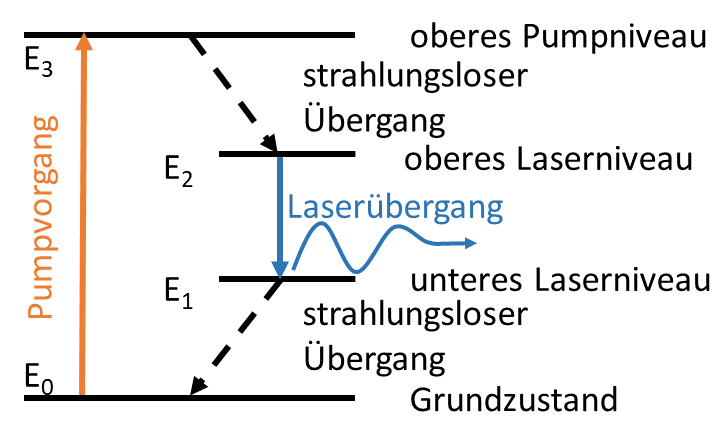
\includegraphics[width=.6\textwidth]{Bilder/Laseruebergang}
\caption{Laserübergang eines Vier-Niveau-Systems.}
\label{Laseruebergang}
\end{figure}
\subsection{Lasing in Nanodrähten}
Nanodrähte aus ZnO sind aufgrund ihrer Materialeigenschaften ein aktives Medium und stellen gleichzeitig mit ihren Wellenleitereigenschaften sowie ihrer durch die hohe Brechzahl bedingte Reflexion an den Endfacetten einen Resonator dar. Dabei spielen die jeweils reflektierten Mode und der Durchmesser des Drahtes eine große Rolle, da sich diese auf den effektiven Brechungsindex auswirken \cite{Maslov.2003}. Im EHP-Zustand bilden Energiezustände mit hohem $\vec{\textbf{k}}$-Vektor im Valenz- und Leitungsband die Pumpniveaus, bei einer Absorption von Photonen mit E$_{\text{Photon}}>$E$_{\text{g}}$. Die so entstandenen Ladungsträger relaxieren durch die in \autoref{ExAn} beschriebenen Streuprozesse innerhalb von hundert Femtosekunden zu den jeweiligen Bandkanten nahe $\vec{\textbf{k}}=$0, wo der eigentliche strahlende Lasingübergang mit höheren Lebensdauern stattfindet \cite{Kneubuhl.2008}. Dieses System lässt sich als Vier-Niveau-System beschreiben \cite{Geburt.Diss}. Eine Inversion kann sich also bei genügend hohen Pumpraten einstellen. 
\subsubsection{Optische Verstärkung}
\label{verst}
Bei der Bewegung durch einen Nanodraht verliert eine elektromagnetische Welle durch Wellenleitung, Absorption, Streuverluste sowie bei der Reflexion an den Endfacetten an Intensität. Die Schwächung der Intensität innerhalb des Materials wird durch das Lambert-Beer'sche Gesetz beschrieben
\begin{equation}
I(\lambda , l)=I_0 \cdot e^{- \alpha(\lambda)\cdot l} \text{ ,}
\end{equation}
mit der Ausgangsintensität I$_{\text{0}}$, dem wellenlängenabhängigen Absorptionskoeffizienten $\upalpha (\uplambda)$ und der vom Licht zurückgelegten Strecke im Material l \cite{Eichhorn.2013}. Bei zunehmenden Anregungsdichten verringert sich der Absorptionskoeffizient $\upalpha (\uplambda)$ für die betreffenden Wellenlängen der Anregung und kann im Zustand des EHP sogar negative Werte annehmen; es findet eine Verstärkung statt, die als verstärkte spontane Emission (engl. \textit{amplified spontaneous emission}, kurz \textit{ASE}) bekannt ist.
Es gilt dann
\begin{equation}
&g(\lambda)=-\alpha(\lambda) \qquad \qquad \qquad \text{ und }	&I(\lambda , l)=I_0 \cdot e^{g(\lambda)\cdot l} \text{ ,}
\end{equation} 
mit der Materialverstärkung $\text{g}(\uplambda$), deren spektraler Verlauf in der \autoref{moden} dargestellt wird. Statt nun mit zunehmender Strecke an Intensität zu verlieren, steigt die Intensität exponentiell an. Für Photonen mit Energien $\text{E}_\text{Photon}<\text{E}_\text{g}$ bleibt das Material transparent, es findet weder Absorption noch Verstärkung statt. Mit erreichen der Bandlückenenergie wächst die Verstärkung an. Der Verlauf ist gegeben durch die Fermifunktionen der Elektronen $\text{f}_\text{e}(\text{E})$ und Löcher $\text{f}_\text{h}(\text{E})$ sowie der kombinierten Zustandsdichte der Bänder D$_\text{CDOS}$(E) (engl. \textit{combined desity of states}, kurz \textit{CDOS})\cite{Klingshirn.2007}:
\begin{equation}
g(E) \sim (f_e(E) +f_h(E)-1) \cdot D_{CDOS}(E) \text{ .}
\end{equation}
Am sogenannten Transparenzpunkt wird die Verstärkung $\text{g}(\text{E}_\text{transp.})= 0$, er markiert die Energie des höchsten angeregten Zustands $\upmu$, alle Photonen höherer Energie unterliegen einer starken Absorption. Typische Werte für die maximale Verstärkung für ZnO sind $\text{g} = 7\cdot$10$^\text{3}\text{cm}^\text{-1}$ \cite{Bohnert.1980}.
\begin{figure}[h]
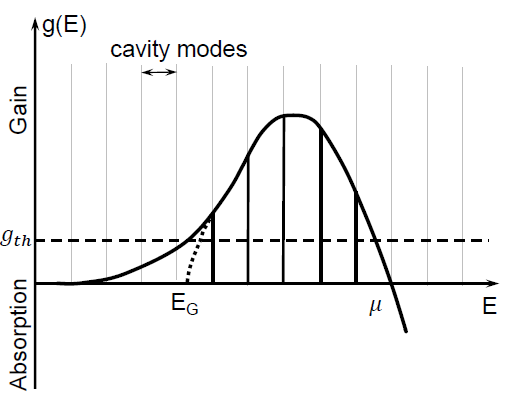
\includegraphics[width=0.4\textwidth]{Bilder/moden}
\caption[Verstärkungsspektrum eines Halbleiters]{Verstärkungsspektrum eines Halbleiters zwischen $\text{E}_\text{g}$ und $\upmu$. Dunkel dargestellt sind die Resonatormoden, deren optische Verstärkung ausreicht, um Lasing oberhalb einer Schwelle g$_{th}$ zu erreichen (aus \cite{Zapf.Master}).}
\label{moden}
\end{figure}
Die Materialverstärkung $\text{g}(\text{E})$ ist experimentell nicht direkt zugänglich, sondern nur die\textit{ modale Verstärkung} $\text{g}_\text{mod}(\text{E})$. Die modale Verstärkung beschreibt die Verstärkung, die das Licht einer bestimmten Mode erfährt, während sie durch das Material propagiert. Sie ist das Produkt der Materialverstärkung mit einem Einschlussfaktor $\Upgamma$ \cite{Richters.2012}, der den räumlichen Überlapp zwischen Lichtwelle und Material beschreibt. 
\begin{equation}
&g_{mod}(E)=\Gamma \cdot g(E) \qquad \qquad \qquad \text{mit } &\Gamma \in [0,1] \text{ .}
\end{equation}
Die modale Verstärkung ist also in der Regel kleiner als die eigentliche Materialverstärkung. Für größere Durchmesser von Nanodrähten kann jedoch $ \Upgamma \approx 1,2$ annehmen \cite{Richters.Diss}, da das Licht in Moden höherer Ordnungen, die nicht parallel zur Längsachse liegen, propagieren kann. Durch diesen ``Zickzackkurs'' legt das Licht einen effektiven Weg im Nanodraht zurück, der größer ist als seine eigentliche Länge \cite{Maslov.2004}. Nach der Definition des Einschlussfaktors für planare Wellen ergibt sich der höhere Wert.\\ 
Laseremission kann stattfinden, sobald die modale Verstärkung im Material die auftretenden Verluste ausgleicht oder überkompensiert, sprich der Schwellwert $\text{g}_\text{th}$(E) (engl. \textit{threshold}) erreicht ist:
\begin{equation}
g_{mod}(E)\leq g_{thres.} = \alpha (E)+ \alpha_R(E) +\alpha_W(E)
\end{equation}
mit den Absorptions- und Reflexionsverlusten $\upalpha (\text{E})$, den Wellenleitungsverlusten $\upalpha_\text{W}(\text{E})$ und den Streuverlusten $\upalpha_\text{Str}(\text{E})$, wobei der Verlust durch Reflexion an den Endfacetten gegeben ist durch:
\begin{equation}
\alpha(E)=\frac{1}{2L}\cdot ln\left(\frac{1}{R_1(E)\cdot R_2(E)}\right)
\end{equation}
mit der Länge L des Resonators und den Reflexivitäten $\text{R}_\text{1,2}$ .
\subsubsection{Nanorähte als Lichtwellenleiter}
Halbleiternanodrähte fungieren, ob ihres hohen Brechungsindex ($\text{n}_\text{NW} \gtrsim 2.5$) verglichen mit ihrer Umgebung ($\text{n}_\text{sur.} \approx 1...1.5$), als Stufenindexfaser, die die vollständige Wellenleitung der Lichtwelle innerhalb der Faser gestattet und somit das Austreten von Licht orthogonal zur Längsachse des Nanodrahtes unterdrückt \cite{Yao.2009}. Hierbei dient der Nanodraht als eigentlicher Kern, das umgebende Medium (Vakuum, Luft, Substrat, ...) als Mantel; dieses System lässt sich als Lichtwellenleiter beschreiben \cite{Pan.2005}. Eine große Rolle hierbei spielt der Einschlussfaktor $\Upgamma$. Dieser ist generell für Nanodrähte höher als für konvenionelle, makroskopische Glasfasern ($\Upgamma_\text{NW} \approx$ 1). Nanodrähte, deren Durchmesser einen Wert $\text{d}_\text{min}\lesssim \uplambda / \text{n}_\text{NW}$ unterschreitet, schießen das Licht nicht mehr vollständig ein, sodass sich ein Teil der Welle außerhalb des Drahtes als evaneszente Welle fortsetzt \cite{Voss.2007}. Dieser Verlauf geht einher mit starken Verlusten in der Lichtwellenleitung. Vor allem für Nanodrähte, die auf einem Substrat aufgebracht sind, spielt dies eine große Rolle. Durch den vergleichsweise hohen Brechungsindex $\text{n}_\text{Substr.} \approx 1.5$ wird der Einschlussfaktor gegenüber dem Substrat stark vermindert, so dass die Moden zunehmend in das Substrat propagieren. So spielt das Substrat für größere Durchmesser $\text{d} \geq \text{d}_\text{min}$ eine kleine Rolle verglichen mit den Auswirkungen des Substrats auf kleinere Durchmesser der Nanodrähte. So findet sich unter d$\approx$ 175 nm nur noch die Grundmode, die für d< 125nm dann auch verschwindet (s. \autoref{abhd}) \cite{Roeder.Diss}.\\
Man unterscheidet bei der Lichtwellenleitung in Halbleiternanodrähten zwischen aktivem und passivem Transport. Der aktive Transport bezieht sich auf Wellenlängen größer als die Bandlücke, die durch Exziton-Polaritonen weitertransportiert werden und dadurch einer wegstreckenabhängigen Rotverschiebung im Material unterliegen\cite{Pan.2005}. Der passive Transport bezieht sich auf Wellenlängen unterhalb der Bandlücke und der Urbach-Ausläufer, bei denen – konventionell, wie in Glasfasern – das Licht entkoppelt von der Exziton-Polariton Wechselwirkung durch den Lichtwellenleiter propagiert \cite{Klingshirn.2007}.
\begin{figure}
\centering
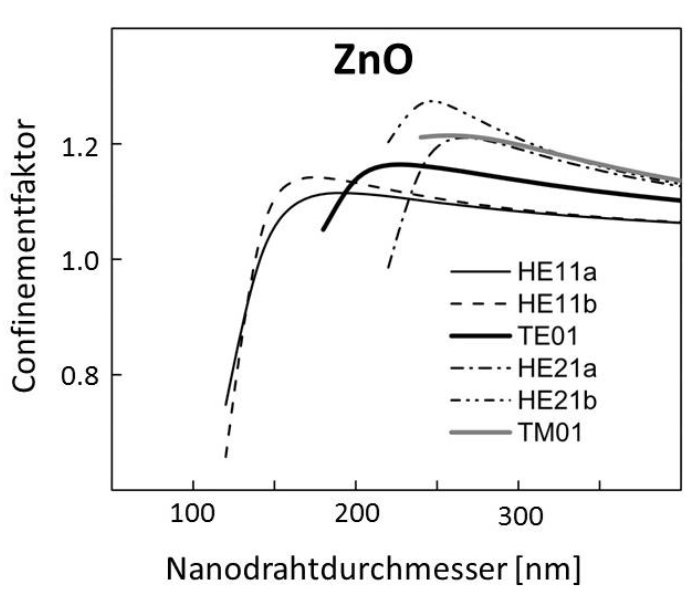
\includegraphics[width=.4\textwidth]{Bilder/abhd}
\caption[Abhängigkeit des Einschlussfaktors von der Nanodrahtdicke]{Simulierter Verlauf der Abhängigkeit des Einschlussfaktors von der Dicke des Nanodrahtes für ZnO. (aus \cite{Zimmler.2010})}
\label{abhd}
\end{figure}
\subsubsection{Fabry-Pérot-Moden}
Aufgrund seiner stabförmigen Geometrie mit den reflektierenden Endfacetten, können Nanodrähte als \textit{Fabry-Pérot-Resonator} (kurz. \textit{FP}) dienen \cite{Zimmler.2008}. Durch die Reflexion an den Endfacetten entsteht im Material eine Interferenz der einlaufenden mit der reflektierten Welle, so dass es zu stehenden Wellen mit definierten Frequenzen entsprechend der Resonanzbedingung 
\begin{equation}
&\lambda_N=\frac{2L\cdot n(\lambda)}{N} \text{ ,} &\Delta \lambda= \frac{1}{L}\left[\frac{\lambda^2}{2}\left(n(\lambda)-\lambda\cdot\frac{dn(\lambda)}{d\lambda}\right)^{-1}\right]
\end{equation}
mit der Wellenlänge $\uplambda_\text{N}$, der Länge des Resonators L, der Dispersion dn/d$\uplambda$, dem Brechungsindex n($\uplambda)$ sowie der Modennummer $\text{N} \in \mathbb{N}$ kommt; alle weiteren Frequenzen interferieren destruktiv. Da jedoch nicht alle Moden eine Verstärkung erfahren (s. \autoref{moden}) ist N begrenzt auf die Bereiche $\text{g}(\text{E})>\text{g}_\text{thres.}$. Der Modenabstand $\Updelta \uplambda$ ergibt sich unter Berücksichtigung der Dispersion, die miteinbezogen werden muss, da sich der Brechungsindex von Mode zu Mode verändert.
\subsubsection{Feldverteilung optischer Moden}
Neben den longitudinalen FP-Lasing-Moden spielt die Feldverteilung in der Ebene senkrecht zur Nanodrahtachse ebenso eine herausgehobene Rolle. Sie ist gegeben durch die Transversalmoden. Diese gliedern sich in transversal-elektrische ($\text{TE}_\text{pl}$), transversal-magnetische ($\text{TM}_\text{pl}$) sowie ihre hybridisierten Moden ($\text{HE}_\text{mpl}$ bzw. $\text{EH}_\text{pl}$). In der $\text{TE}_\text{pl}$-Mode existiert nur die elektrische Feldkomponente senkrecht zur Ausbreitungsrichtung des Lichtes $\vec{\textbf{k}}$, während die magnetische Feldkomponente in Ausbreitungsrichtung zeigt; bei der $\text{TM}_\text{pl}$-Mode ist es umgekehrt. Die Hybridmoden enthalten sowohl elektrische als auch magnetische Komponenten und zeigen in Ausbreitungsrichtung $\vec{\textbf{k}}$ \cite{Kneubuhl.2008}. Die simmulierten Feldverteilungen dieser Moden sind abgebildet in \autoref{Moden2}. Die Indizes p, l bezeichnen die Modenzahl bezüglich der Radial- und der Winkel-Komponenten des Feldes. 
\begin{figure}[hb]
\centering
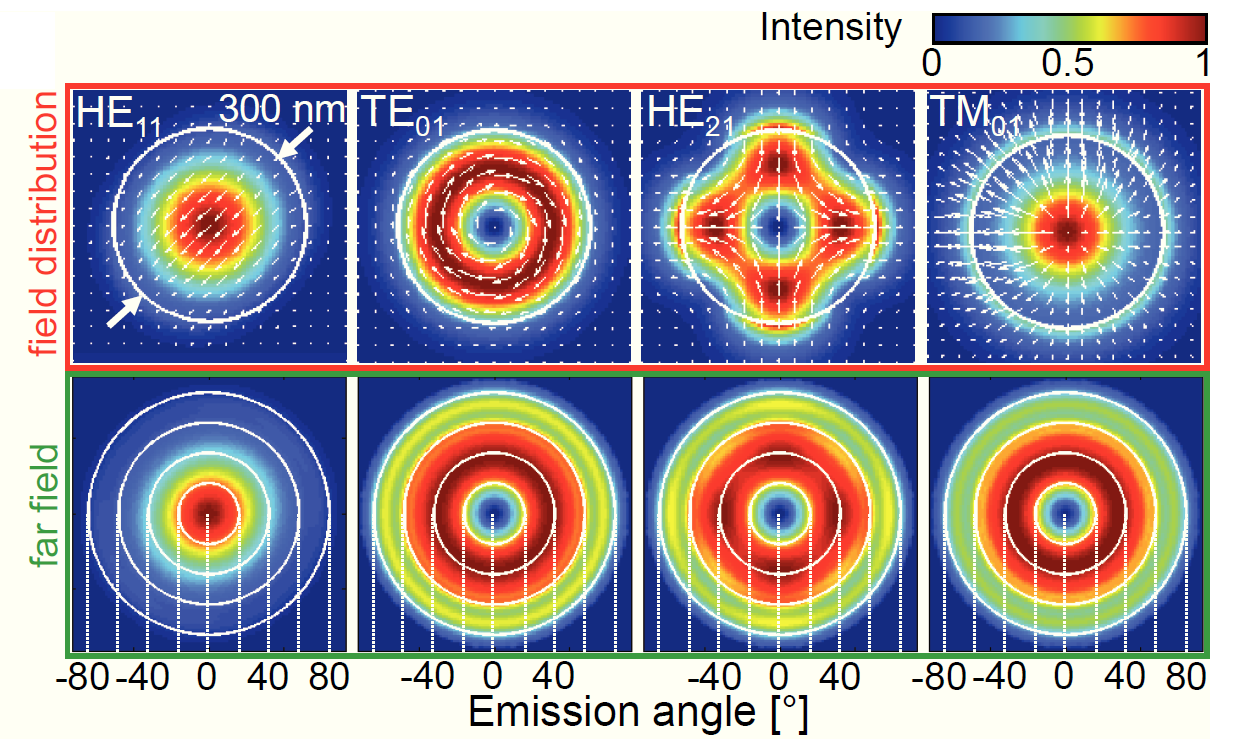
\includegraphics[width=.5\textwidth]{Bilder/moden2}
\caption[Feldverteilung der Moden eines ZnO-Nanodrahtes]{Simulierte Feldverteilungen der vier niedrigsten Moden eines zylindrischen ZnO-Nanodrahtes mit 300 nm Durchmesser. Oben die Verteilung im Nanodraht, unten die Emission ins Fernfeld. (aus \cite{Roeder.Diss})}
\label{Moden2}
\end{figure}
%\subsubsection{Feldverteilung plasmonischer Hybridmoden}
%Für Nanodrähte auf plasmonisch aktiven Substraten erscheinen zusätzlich zu den photonischen Moden zusätzliche plasminosche Hybridmoden (engl. \textit{hybrid surface plasmonic mode} kurz \textit{HSP}). Da der elektrische Feldvektor orthogonal zur Oberfläche eine Grundvoraussetzung für das Entstehen der SSP ist, können diese nicht als TE-Mode vorliegen, sondern ausschließlich für die TM Polarisation \cite{Maier.2010}. 
%\textbf{!!Hier müssen wir die Simulationen der Theoretiker abwarten!!}
%\subsubsection{Einschluss plasmonischer Moden}
\subsubsection{Leistungscharakteristik}
Um Lasingverhalten von ASE (s. \autoref{verst}) zu unterscheiden, muss ein Vergleich mit einem theoretischen Modell gezogen werden. Da beim Lasing in Nanodrähten verschiedenste Moden gleichzeitig auftreten und um Verstärkung konkurrieren, können die Moden nicht einzeln, sondern nur als Gesamtheit betrachtet werden. Etabliert hat sich hierbei das Multimoden-Laser-Modell nach Casperson (1975) \cite{Casperson.1975}. Es zeigt analytisch die Abhängigkeit der gesamten emittierten Strahlungsleistung $\text{x}_\text{t}$ vom Verstärkungs-Verlust-Verhältnis $\text{r}$ pro Resonatorumlauf. Die auf einen Resonatorspiegel auftreffende Gesamtintensität aller konkurrierender Lasingmoden ist gegeben durch
\begin{equation}
&x_t=\frac{r(1+x)^{-1}x_0}{\sqrt{1-r(1+x)^-{1}}} \text ,]\qquad \quad \text{mit }&x_0=x\left[\sqrt{\frac{1+x}{1+x-r}}-1 \right] \text{ .}
\end{equation}
Hierbei stellt $\text{x}_\text{0}$ ein Maß für den Anteil spontaner Emission in den Lasingmoden dar. Für jedes r wird der Parameter x aus der impliziten Gleichung bestimmt. Obige Gleichungen gelten für die Näherung kleiner Frequenzabstände der longitudinalen Moden gegenüber der Linienbreite des Verstärkungsprofils. An der Laserschwelle gilt $\text{r}= 1$. Es ergibt sich ein S-förmiger Verlauf bei einer doppellogarithmischen Darstellung. Unterhalb der Lasingschwelle nimmt die spontane Emission als Funktion der Pumpleistung bzw. des Verstärkungs-Verlust-Verhältnisses linear zu. Im Bereich um die Lasingschwelle in ein starkes nicht-lineares Verhalten der spontanen Emission dadurch gegeben, dass nun eine Verstärkung einsetzt. Im Lasingbereich ist der Zusammenhang zwischen gepumpter und emittierter Leistung dann wieder linear.
\begin{figure}[h]
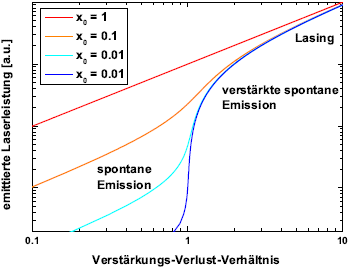
\includegraphics[width=0.5\textwidth]{Bilder/casperson}
\caption[Lasercharakteristik]{Doppellogarithmische Darstellung der Abhängigkeit der emittierten Strahlungsleistung als Funktion der Pumpleistung bzw. des Verstärkungs-Verlust-Verhältnisses. (nach \cite{Casperson.1975})}
\label{casperson}
\end{figure}
\section{Polarisation und Stokes-Parameter}
\subsection{Polarisationsrichtung von elektromagnetischen Wellen}
Neben der Intensität und der Wellenlänge trägt eine elektromagnetische Welle eine weitere nicht direkt messbare Information – die Polarisation.
Aus der Lösung der Maxwell-Gleichungen ergibt sich für den elektrischen Feldanteil im Vakuum 
\begin{equation}
\vec{\textit{\textbf{E}}}(\vec{\textit{\textbf{r}}},t)=E_0 e^{i(\vec{\textit{\textbf{k}}} \cdot \vec{\textit{\textbf{r}}} -\omega t)} \vec{\textit{\textbf{e}}_{\textit{\textbf{r}}}}
\end{equation}
mit Ausbreitungsrichtung z folgt daher für die x- und y-Komponente des Feldes
\begin{equation}
E_x(\vec{\textit{\textbf{z}}},t)&=E_{0,x} cos(\vec{\textit{\textbf{k}}} \cdot \vec{\textit{\textbf{z}}} - \omega t)\\
E_y(\vec{\textit{\textbf{z}}},t)&=E_{0,y} cos(\vec{\textit{\textbf{k}}} \cdot \vec{\textit{\textbf{z}}} - \omega t + \delta)
\end{equation}
mit der Phasenverschiebung $\updelta$ zwischen den beiden Komponenten. Für $\updelta= \text{n}\uppi$ ($\text{n} \in \mathbb{Z}$) erfolgt eine lineare Polarisation in Ausbreitungsrichtung, für $\updelta\neq$ n$\uppi$ ergibt sich unter Benutzung des Additionssatzes des Kosinus eine Polarisationsellipse
\begin{equation}
\left( \frac{E_x(\vec{\textit{\textbf{z}}},t)}{E_{0,x}}\right)^2 +\left( \frac{E_y(\vec{\textit{\textbf{z}}},t)}{E_{0,y}} \right)^2- 2\frac{E_x(\vec{\textit{\textbf{z}}},t)E_y(\vec{\textit{\textbf{z}}},t)}{E_{0,x}E_{0,y}}cos(\delta)=sin^2(\delta)
\end{equation}
einschließlich des Spezialfalles $\updelta = \pm \frac{\uppi}{\text{2}}$ und $\text{E}_\text{0,x}=$ E$_\text{0,y}$ in dem sich zirkular polarisiertes Licht ergibt. Die Hauptachsen der Ellipse müssen dabei nicht auf denen des Koordinatensystems liegen, sondern können um einen Winkel $\uppsi$ verschoben sein. Eine aussführliche Beschreibung findet sich bei Collett (1993) \cite{Collett.1993}. Unpolarisiertes Licht besitzt im Gegensatz zu polarisiertem,   weder ein zeitlich konstantes Phasen- noch Amplitudenverhältnis und kann somit aus Überlagerung vieler linear polarisierter Wellen aufgefasst werden.
\subsection{Stokes-Parameter}
Die Polarisation einer elektromagnetischen Wellen ist nicht direkt messbar, sie kann aber unter anderem mithilfe eines linearen Polarisators und eines $\uplambda$/4- Plättchens über die Intensität rekonstruiert werden (s. \autoref{Mess.Stokes}). Die Intensität ist darstellbar als zeitliche Mittellung der quadrierten Feldelemente, so dass
\begin{equation}
I(\theta)= \underbrace{(E_{0,x}^2+E_{0,y}^2)^2}_{=S_0^2}=\frac{1}{2}[\underbrace{(E_{0,x}^2-E_{0,y}^2)^2}_{=S_1^2} &+ \underbrace{(2E_{0,x}E_{0,y}cos(\delta))^2}_{=S_2^2}+\underbrace{(2E_{0,x}E_{0,y}sin(\delta))^2}_{=S_3^2}]
\label{StokesGl}
\end{equation}
gilt. Die Parameter $\text{S}_\text{0...3}$ werden nach dem Entwickler dieses Formalismus \textit{Stokes-Parameter} genannt \cite{Stokes.1851}.
S$_\text{0}$ beschreibt hierbei die Gesamtintensität, die sich aufgliedert:
\begin{itemize}
\item $\text{S}_\text{1}$, die Differenz zwischen horizontal und vertikal polarisiertem Licht;
\item $\text{S}_\text{2}$, die Differenz zwischen $+45^\circ$ und $-45^\circ$ polarisiertem Licht;
\item sowie in $\text{}S_\text{3}$, die Differenz aus rechts- und linkszirkular polarisiertem Licht.
\end{itemize}
Für Licht mit Anteilen an polarisierten und unpolarisierten Licht geht die obige Gleichung in eine Ungleichung über in
\begin{equation}
S_0^2 &\leq S_1^2 + S_2^2 + S_3^2\\
S_0^2 \cdot DOP^2&= S_1^2 + S_2^2 + S_3^2\\
\Rightarrow DOP&=\frac{\sqrt{S_1^2+S_2^2+S_3^2}}{S_0} &DOP \in [0,1] \text{ .}
\end{equation}
Entsprechend wird ein Korrekturfaktor eingefügt, der die Ungleichung zurück in eine Gleichung überführt. Dieser Faktor DOP wird \textit{Polarisationsgrad} (engl. \textit{degree of polarization}, kurz \textit{DOP}) genannt. Oftmals werden die Stokes-Parameter aus praktischen Gründen als Vektor dargestellt. Unvollständig polarisiertes Licht findet also folgende Darstellung:
\begin{equation}
\left(
\begin{matrix}
S_0 \\ 
S_1 \\ 
S_2 \\ 
S_3
\end{matrix} 
\right)
= (1-DOP)
\left(
\begin{matrix}
S_0 \\ 
0 \\ 
0 \\ 
0
\end{matrix} 
\right)_{UP}
+ DOP
\left(
\begin{matrix}
S_0 \\ 
S_1 \\ 
S_2 \\ 
S_3
\end{matrix} 
\right)_{P} \text{ ,}
\end{equation}
mit der Aufspaltung in die unpolarisierten und vollständig polarisierten Anteile \cite{Schaefer.2007}. Die Drehung $\Uppsi$ der Polarisationsellipse gegenüber dem Koordinatensystem, sowie die Elliptizität $\upchi$ sind gegeben durch die Verhältnisse der Stokes-Parameter:
\begin{equation}
\Psi &=\frac{1}{2}arctan\left(\frac{S_2}{S_1}\right)\qquad \text{mit }\qquad\qquad  0 \leq \Psi \leq \pi \text{ ,}\\
\chi &=\frac{1}{2}arcsin\left(\frac{S_3}{S_0}\right)\qquad \text{mit}\qquad\quad  -\frac{\pi}{4} \leq \chi \leq \frac{\pi}{4} \text{ .}
\end{equation}
\section{Magnetismus und Spinpolarisation}
Elektronen besitzen, wie alle Fermionen, einen halbzahligen Spin  $\textbf{s}= \frac{1}{2}$, sowie ein magnetisches Dipolmoment $\vec{\boldsymbol{\upmu}}_{\textbf{s}}=\text{g}_\text{e}\upmu_\text{B}\frac{\vec{\textbf{s}}}{\hbar}$. Es ist also möglich, den Spin mithilfe eines Magnetfeldes auszurichten \cite{Gross.2014}. Die Ausrichtung des Elektronenspins ist bei der Rekombination mit einem Loch und der daraus resultierenden Emission eines Photons mitbestimmend für dessen Polarisationsrichtung (s.\autoref{AusR}), sie spielt folglich eine wichtige Rolle im Verständnis der Polarisierbarkeit der Licht- und Laseremission und soll im Folgenden kurz erläutert werden.
%\subsection{Spin-Bahn-Wechselwirkung}
%Im Atom koppelt der Spin der Elektronen an das Magnetfeld des Kerns. Dieses wiederum hängt maßgeblich vom Bahndrehimpuls des Elektrons ab, man spricht von der sog. \textit{Spin-Bahn-Kopplung}. Sie spielt vor allem bei Atomen größerer Masse eine herausragende Rolle, da die gegenseitige elektrostatische Störung der Elektronen vernachlässigbar wird. Spin und Bahndrehimpuls der einzelnen Elektronen koppeln zum Gesamtdrehimpulse $\vec{\textbf{s}}_{\textbf{i}} + \vec{\textbf{l}}_{\textbf{i}}= \vec{\textbf{j}}_{\textbf{i}}$. Jene koppeln sich zum Gesamtdrehimpuls $\vec{\textbf{J}}$ des Atoms zusammen $ \vec{\textbf{J}}=\sum_i \vec{\textbf{j}}_{\textbf{i}}$ . Hierbei sind nur Elektronen unbesetzter Schalen zu berücksichtigen, da der Gesamtdrehimpuls einer abgeschlossenen Schale sich zu Null ergibt. Für Atome kleiner Kernladungszahl kann die Spin-Bahn-Wechselwirkung vernachlässigt werden, hier spielt die spinunabhängige Coulomb-Wechselwirkung der Elektronen untereinander die entscheidende Rolle. Beschrieben wird dies durch die LS-Kopplung, bei der sich die Bahndrehimpulse und Spins getrennt voneinander aufsummieren. Es gilt $ \vec{\textbf{L}}=\sum_i \vec{\textbf{l}}_{\textbf{i}}$ und $ \vec{\textbf{S}}=\sum_i \vec{\textbf{s}}_{\textbf{i}}$, beide Gesamtgrößen koppeln dann zum Gesamtdrehimpuls $ \vec{\textbf{J}}= \vec{\textbf{L}} +  \vec{\textbf{S}}$, der eine Erhaltungsgröße darstellt. Für die Drehimpulsquantenzahl gilt $\text{l}=\text{0,1,2..}<\text{n}$, mit der Hauptquantenzahl n. Oftmals werden für den Wert dieser Quantenzahl historisch geprägte Buchstaben verwendet, so wird $\text{l}=\text{0}$ als s-Zustand bezeichnet, $\text{l}=1$ als p-Zustand, $\text{l}=\text{2}$ als d-Zustand, usw. Eine weitere wichtige Quantenzahl ist die magnetische Quantenzahl mit $\text{m}_\text{l}=\text{-l, } \text{-(l-1), }..,\text{(l-1), }\text{l}$, die die zusätzliche Energie der Elektronen beim Anlegen eines magnetischen Feldes beschreibt.
\subsection{Lamorpräzession und Zeeman-Aufspaltung}
\label{Zee}
Entsprechend seines magnetischen Dipolmoments $\vec{\textbf{$\upmu$}}$ erfährt ein Atom oder Elektron in einem Magnetfeld  $\vec{\textbf{B}}$ ein Drehmoment
\begin{equation}
&\vec{\textit{\textbf{M}}}= \vec{\textbf{$\mu$}} \times \vec{\textit{\textbf{B}}} \qquad \qquad\qquad \text{ und } 
&\vec{\textbf{$\mu$}}=g_j \frac{q}{2m} \vec{\textit{\textbf{j}}}
\end{equation}
mit dem Landé-Faktor $\text{g}_\text{j}$, der Ladung q und der Masse m des Teilchens \cite{Gross.2014}. Dieses Drehmoment bewirkt, dass der Dipol parallel zum Feld ausgerichtet wird. Als Folge der Drehimpulserhaltung  wird dem Teilchen eine Präzessionsbewegung aufgezwungen. Die Frequenz dieser Bewegung wird als \textit{Lamor-Frequenz} $\upomega_\text{L}$ bezeichnet und gibt die zeitliche Änderung des Drehimpulses wieder
\begin{equation}
&\frac{d\vec{\textit{\textbf{J}}}}{dt}= \vec{\textbf{$\omega$}}_{\textit{\textit{\textbf{L}}}} \times \vec{\textit{\textbf{J}}} \qquad \qquad\qquad \text{ und }
&\vec{\textbf{$\omega$}}_{\textbf{L}}= g_j \frac{q}{2m} \vec{\textit{\textbf{B}}}.
\end{equation}
Da es bei Elektronen im quantenmechanischen Sinne nur zwei Ausrichtung des Spins gibt kann diese Präzessionsbewegung nicht als kontinuierliche Drehung verstanden werden, sondern als Zeit- oder Enselblemittel der Superposition vieler teilnehmender Elektronen. Im Fall der LS-Kopplung führt dieser zusätzliche Energieterm zu einer Aufspaltung der entarteten Energieniveaus nach der Quantenzahl $\text{m}_\text{j}$ in 2J+1 äquidistante Energieniveaus. Dieser Effekt ist als \textit{anormaler Zeeman-Effekt} bekannt, der wiederum als Spezialfall $\text{m}_\text{j}=\text{m}_\text{l}$ bei $\vec{\textbf{S}}=0$ den \textit{normalen Zeeman-Effekt} beinhaltet \cite{Gross.2014}. Die Energieaufspaltung beträgt
\begin{equation}
\Delta E=g_j m_j \frac{q\hbar}{2m} B.
\end{equation}
Bei sehr hohen Magnetfeldern findet eine Entkopplung von Spin und Bahndrehimpuls statt, die Niveaus verschieben sich weiter und liegen nicht mehr äquidistant; das Dipolmoment wird zu $\vec{\textbf{$\upmu$}}=\frac{\text{q}}{\text{2m}}(\text{g}_\text{L}\vec{\textbf{L}}+\text{g}_\text{s}\vec{\textbf{S}})$. Dieser Effekt ist als \textit{Paschen-Back-Effekt} bekannt \cite{Gross.2014}. 
\subsection{Auswahlregeln und Spinpolarisation}
\label{AusR}
Die Emission oder Absorption von Photonen folgt strengen Regeln; die Übergangswahrscheinlichkeiten sind durch \textit{Fermis Goldene Regel} gegeben \cite{Dirac.1927}. Für den optischen Dipolübergang zur Erzeugung oder Vernichtung eines Exzitons gilt die Erhaltung des Gesamtdrehimpulses $\vec{\textbf{J}}=\vec{\textbf{L}}+\vec{\textbf{S}}$. Da das Photon selbst einen Spin $\vec{\textbf{s}}$ und somit einen Gesamtdrehimpuls von $|\vec{\textbf{j}}|=|\vec{\textbf{s}}|=\hbar$ trägt, können nur solche Übergange mit $|\Updelta \vec{\textbf{J}}|=\hbar$ stattfinden. Entsprechend sind auch nur solche Übergänge der Magnetquantenzahl $\Updelta \text{m}_\text{j}=\text{0,}\pm \text{1}$ erlaubt. Hierbei gibt $\Updelta\text{m}_\text{j}$ die Polarisierungsrichtung des Lichtes an: $\Updelta\text{m}_\text{j}=\text{0}$ für linear polarisiertes ($\pi$), $\Updelta\text{m}_\text{j}=\pm\text{1}$ für rechts- ($\sigma^{+}$) bzw. linkszirkulär ($\sigma^{-}$) polarisiertes Licht. Diese Regeln gilt es nun in Relation zu der Bandstruktur zu setzten.\\
Das Leitungsband in Zinkoxid hat den Drehimpuls $\text{j}=\text{s}=\frac{\hbar}{\text{2}}$ bei $\text{l}=\text{0}$. Das Valenzband ($\text{l}=\text{1}$) mit dem Spin $\text{s}=\frac{1}{2}$
ist in drei Subbänder aufgespalten (s. \autoref{ZnOMat}). Das HH-Band besitzt hierbei einen Bahndrehimpuls von $\text{j}=\frac{3}{2}$ mit der Magnetquantenzahl $\text{m}_\text{j}=\frac{3}{2}$, das LH-Band $\text{j}=\frac{3}{2}$ bei $\text{m}_\text{j}=\frac{1}{2}$ und das SO-Band $\text{j}=\frac{1}{2}$ bei $\text{m}_\text{j}=\frac{1}{2}$. Diese vier Bänder sind zusätzlich wegen $\text{s}_\text{z}=\pm\frac{1}{2}$ jeweils doppelt entartet. So ergeben sich die in \autoref{Ausw} dargestellten möglichen Übergänge mit verschieden polarisiertem Licht.
\begin{figure}[h]
\centering
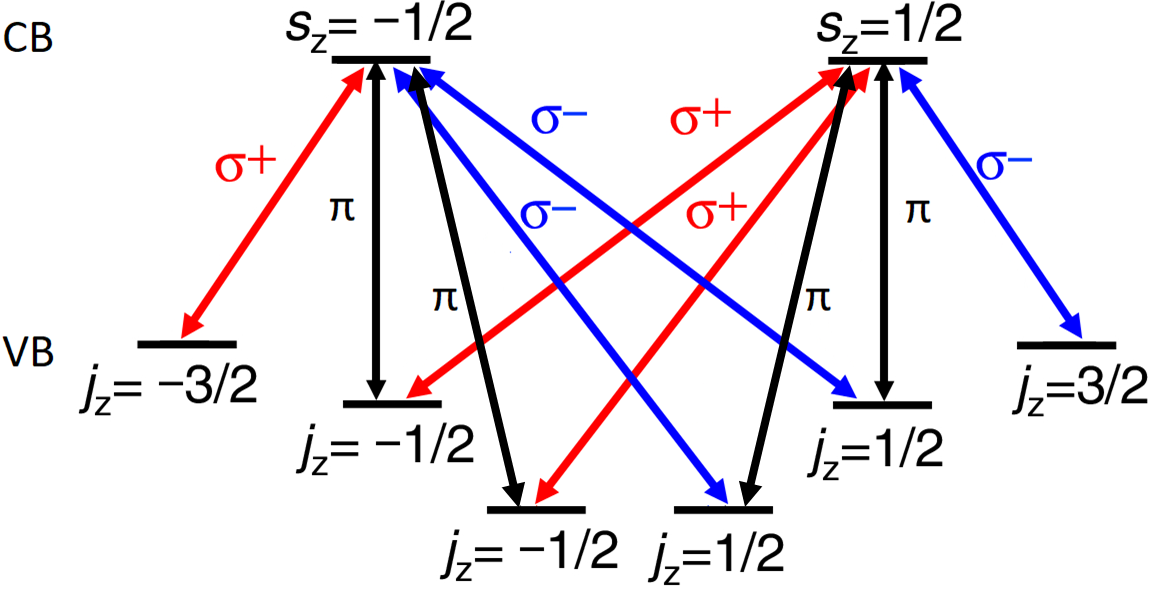
\includegraphics[width=.5\textwidth]{Bilder/ausw}
\caption[Auswahlregeln]{Mögliche Übergänge von den Valenzbändern in das Leitungsband unter Berücksichtigung der Auswahlregeln.}
\label{Ausw}
\end{figure}
Um nun eine Spinpolarisation zu generieren, muss einer der beiden Leitungsbandzuständen bevorzugt bevölkert werden. Die Spinpolarisation ist also eine Abweichung aus der Gleichverteilung und berechnet sich wie folgt
\begin{equation}
P=100\%\cdot \frac{\left| N_\uparrow- N_\downarrow\right|}{N_\uparrow+ N_\downarrow}
\end{equation}
mit der Anzahl N der jeweils Spin-Up und Spin-Down ausgerichteten  Elektronen.
\subsection{Spinrelaxation und Spindephasierung}
Injiziert man eine Spinpolarisation in ein angeregtes Elektronensystem, so kommt es auf die Zeitdauer an, in der dieser Zustand erhalten bleibt, verglichen mit der Zeitdauer der Rekombination, damit diese Spinpolarisation einen Einfluss auf die Emissionscharakteristik haben kann. Es gilt
\begin{equation}
P=\frac{P_0}{1+ \frac{\tau}{\tau_{SR}}}
\end{equation}
mit der Rekombinationszeit der Elektronen $\uptau$ und deren Spinrelaxationszeit $\uptau_\text{SR}$ \cite{Dyakonov.2008}. Die wichtigsten Mechanismen, die zur Relaxation dieser Spinpolarisation führen, sollen in Folgenden betrachtet werden.
\subsubsection{Spinrelaxationszeit T$_\text{1}$}
Die Spinrelaxationszeit $\text{T}_\text{1}$ charakterisiert die Rate, in der ein ausgerichtetes Spinensemble wieder das thermische Gleichgewicht mit der Umgebung erreicht. Es gilt:
\begin{equation}
M_z(t)=M_{z,eq} -\left[ M_{z,eq}-M_z(0)\right]\cdot e^{t/T_1} \text{ ,}
\end{equation}
mit der Magnetisierung in z-Richtung $\text{M}_\text{z}$. T$_\text{1}$ wird auch als longitudinale Relaxationszeit oder entsprechend der maßgeblichen Wechselwirkung als Spin-Gitter-Relaxation bezeichnet \cite{Zutic.2004}.
\subsubsection{Spindekohärenzzeit T$_\text{2}$}
Die Spindekohärenzzeit oder transversale Relaxationszeit T$_\text{2}$ beschreibt die Rate, in der ein mit Lamorfrequenz um ein Magnetfeld präzedierender Spin seine Phase verliert und wird maßgeblich von der Spin-Spin-Wechselwirkung verursacht \cite{Fabian.2007}. Übertragen auf ein Spinensemble findet also eine zunehmende Dephasierung statt. Es gilt:
\begin{equation}
M_{xy}(t)=M_{xy}(0)\cdot e^{-t/T_2} \text{ ,}
\end{equation}
mit der Magnetisierung in der xy-Ebene $\text{M}_\text{xy}$. Obwohl beide Relaxationsmechanismen nicht in direkter Verbindung stehen gilt für die meisten nichtkubischen Gitter die Näherung
\begin{equation}
T_1 = T_2 \text{\cite{Fabian.2007} .}
\end{equation}
\subsubsection{Spindephasierungszeit T$_2^*$}
Je mehr Spins an einem solchen Spinsystem beteiligt sind, desto mehr Möglichkeiten bestehen, diese außer Phase zu bringen. Solche zusätzlichen Dephasierungsmechanismen können beispielsweise Variationen des g-Faktors durch mikroskopische Unregelmäßigkeiten des Kristallfeldes o.ä. entstehen und verursachen eine inhomogene Linienverbreiterungen \cite{Fabian.2007}. Durch diese Mechanismen verkürzt sich die Zeit in der ein Ensemble kohärent bleibt.
\subsubsection{Der Elliott-Yafet-Mechanismus}
Der Elliott-Yafet-Mechanismus (kurz \textit{EYM})\cite{Elliott.1954,Yafet.1963} beschreibt das Zusammenspiel der Spin-Bahn-Wechselwirkung mit einem beliebigen Streuprozess, so z.B. an anderen Elektronen \cite{Boguslawski.1980}, Phononen oder an Gitterdefekten. Es kommt im Leitungsband zu einer Mischung von Spin-Up $\ket{\uparrow}$ und Spin-Down $\ket{\downarrow}$ Zuständen
\begin{equation}
\Psi_{\vec{\textbf{k}},n,\uparrow}(\vec{\textbf{r}})=\left( a_{\vec{\textbf{k}},n}(\vec{\textbf{r}})\ket{\uparrow} + b_{\vec{\textbf{k}},n}(\vec{\textbf{r}})\ket{\downarrow}\right)\cdot e^{i \vec{\textbf{k}}\cdot \vec{\textbf{r}}}\\
\Psi_{\vec{\textbf{k}},n,\downarrow}(\vec{\textbf{r}})=\left( a_{\vec{\textbf{k}},n}(\vec{\textbf{r}})\ket{\downarrow} + b_{\vec{\textbf{k}},n}(\vec{\textbf{r}})\ket{\uparrow}\right)\cdot e^{i \vec{\textbf{k}}\cdot \vec{\textbf{r}}}
\end{equation}
mit dem Bandindex n und $\mid\text{b}_{\vec{\textbf{k}},\text{n}}\mid \ll \mid\text{a}_{\vec{\textbf{k}},\text{n}}\mid$). Bei solchen Mischzuständen bleibt der vorhandene Spin bis zu einem Streuereignis konserviert, erst ein solches kann den Übergang induzieren – man spricht von einem \textit{Spinflip}. Die Effektivität des EYM ist also eng mit der Spinrelaxationszeit $\uptau_\text{SR}$ verknüpft. Es gilt: 
\begin{equation}
\tau_{SR} \propto \tau_{p} \text{ .}
\end{equation}
Diese Beziehung ist charakteristisch für den EYM. %Entsprechend ist der EYM auch stark Temperaturabhängig zumal bei steigenden Temperaturen vermehrt mit Phononen zu rechnen ist. So gilt der Zusammenhang $\frac{1}{\uptau} \propto \text{T}$ bei Temperaturen T größer der Debye-Temperatur $\Uptheta_\text{D}$, für kleinere Temperaturen gilt $\frac{1}{\uptau} \propto \text{T}^\text{5}$.
Der EY-Mechanismus ist vor allem für Halbleiter mit kleinen Bandlücken und großen Spin-Bahn-Aufspaltungen des Valenzbandes effektiv, denn es gilt:
\begin{equation}
\frac{1}{\tau_{SR}}=A \cdot \left(\frac{\Delta_{SO}}{E_g+\Delta_{SO}}\right)^2 \left(\frac{E_k}{E_g}\right)^2  \frac{1}{\tau_p}
\end{equation}
mit einem vom Streuprozess abhängigen numerischen Faktor A, der Bandlücke E$_\text{g}$, der Spin-Bahn-Aufspaltung des Valenzbandes $\Updelta_\text{SO}$, sowie der kinetischen Energie des Elektrons vor dem Stoß E$_\text{k}$. Obgleich ZnO eine vergleichsweise große Bandlücke bei kleiner Aufspaltung des Valenzbandes besitzt, so ist der EYM dominierend für sehr kleine Temperaturen T$\leq$5 K \cite{Buyanova.2010,Whittaker.1996}.
\subsubsection{Der D'yakonov-Perel'-Mechanismus}
Der D'yakonov-Perel'-Mechanismus (kurz \textit{DPM})\cite{Dyakonov.1971} tritt in Materialien ohne Inversionssymmetrie auf, zu denen u.a. auch ZnO zählt. Hierdurch wird die Entartung der Spinzustände aufgehoben, es resultiert ein richtungsabhängiges internes Magnetfeld $\vec{\textbf{B}}(\vec{\textbf{k}}$) in dem der Elektronenspin zu präzedieren beginnt. Wird nun das Elektron nach einer Zeit $\uptau_\text{p}$ gestreut, verändert sich der $\vec{\textbf{k}}$-Vektor und somit die Richtung und die Stärke des effektiven Magnetfeldes, um das der Spin des Elektrons präzediert\cite{Zutic.2004}. Man spricht in diesem Zusammenhang von der Korrelationszeit $\uptau_\text{c}$ innerhalb derer das fluktuierende Magnetfeld sich mittelt und als konstant betrachtet werden kann. Es lassen sich hierbei zwei Fälle unterscheiden: Die Elektonenspins können mindestens einen vollständigen Präzessionszyklus innerhalb der Korrelationszeit durchlaufen, oder eben nicht.
Für den ersten Fall gilt
\begin{equation}
\tau_c \Omega \gg 1
\end{equation}
mit der über $\vec{\textbf{k}}$ gemittelten Präzessionsfrequenz $\Upomega$. Hierdurch dephasieren die Elektronenspins aufgrund der Inhomogenitäten des effektiven Magnetfeldes. Die Spinrelaxationszeit $\uptau_\text{SR}$ ist proportional zur Breite der Verteilung des effektiven Magnetfeldes und somit zur Korrelationszeit $\uptau_\text{c}$, es gilt $\uptau_\text{SR} \approx \uptau_\text{c}$.\\ %Der Prozess ist reversibel \cite{Hu.2002}.
Für den zweiten Fall gilt
\begin{equation}
\tau_c \Omega \ll 1 \text{ .}
\end{equation}
Dieser als \textit{``motional narrowing''}  bekannter Fall wird vom DPM beschrieben, und ähnelt viel mehr der Präzession in einem inhomogenen Magnetfeld. Die Spinrelaxationszeit lässt sich mit dem Modell eines \textit{Random-Walk} abschätzen. Zwischen zwei Streuprozessen präzediert der Spin um den Winkel $\upvarphi=\uptau_\text{c} \Upomega$. Nach einer Zeit t ist der Erwartungswert des quadrierten Drehwinkels $\Braket{\Updelta\upvarphi^\text{2}}$ proportional zur Anzahl der Random-Walk-Schritte $\text{t}/\uptau_\text{c}$ multipliziert mit der quadrierten Schrittweite $(\Upomega \tau_\text{c})^\text{2}$
\begin{equation}
\Braket{\Delta\upvarphi^2} \sim \Omega^2\tau_c t
\end{equation}
Die Spinrelaxationszeit $\uptau_\text{SR}$ ist hierbei über die Bedingung $\Braket{\Updelta\upvarphi^\text{2}} \sim \text{1}$ bei $\text{t}=\uptau_\text{SR}$ gegeben, so dass 
\begin{equation}
\frac{1}{\uptau_{SR}} \sim \Omega^2\tau_c
\end{equation}
folgt. Dieser Zusammenhang ist charakteristisch für den DPM. Die Spinrelaxationszeit steigt also mit der Häufigkeit der Streuprozesse. Generell gilt also $\uptau_\text{SR} \gg \uptau_\text{c}$.  Anschaulich können die Spins dem Wechsel des Magnetfeldes nicht mehr folgen und behalten somit ihre ursprüngliche Orientierung.\\\\
Der DPM ist für Halbleiter ohne Inversionssymmetrie für Temperaturen $\text{T}>\text{5}$ K der dominierende Prozess. Er dominiert in undotierten und n-dotierten Systemen, die die Bedingung des \textit{``motional narrowing''} erfüllen \cite{Zutic.2004}. Zudem wurde von Whittaker et al. (1996) \cite{Whittaker.1996} theoretisch gezeigt, dass \textit{``motional narrowing''} in qualitativ hochwertigen Halbleiter-Mikrokavitäten zu erwarten ist.
\subsubsection{Einfluss eines externen Magnetfelds auf den D'yakonov-Perel'-Mechanismus}
Legt man nun zusätzlich ein homogenes externes Magnetfeld an, präzidieren die Spins  mit der Lamor-Frequenz $\upomega_\text{L}=\text{g}_\text{j}\frac{\text{q}}{\text{2m}}\vec{\textbf{B}}$ um das Magnetfeld $\vec{\textbf{B}}$. Für den Fall eines homogenes internes Feld, bleibt der Spinvektor konstant – Relaxation kann nur über die Inhomogenitäten erfolgen. Liegen die Inhomogenitäten des inneren Magnetfeldes in Richtung des externen Magnetfeldes, so spielt das Vorhandensein des externen Feldes keine Rolle für die transversale Spinrelaxationszeit $\text{T}_\text{2}$, da sich das Feld durch Rotation nicht ändert. Es bleibt bei der charakteristischen Zeit $\text{T}_\text{2} \approx \uptau_\text{SR}$. 
Für die senkrecht zum externen Magnetfeld stehenden Fluktuationen hingegen ergibt sich ein anderes Bild, denn hier rotiert der Spinvektor mit der Lamor-Frequenz durch die Inhomogenitäten. Sie beeinflussen die Spinrelaxation in Richtung des externen Feldes und somit die longitudinale Spinrelaxationszeit $\text{T}_\text{1}$, die damit von der Stärke des externen Magnetfeldes abhängig wird.\\
Für $\uptau_\text{c}\upomega_\text{L} \ll \text{1}$ spielt diese Präzessionsbewegung eine untergeordnete Rolle, da sich das Feld schon zuvor in der Zeit $\uptau_\text{c}$ geändert hat. Für den Fall das $\uptau_\text{c} \upomega_\text{L} \gg \text{1}$ hingegen rotiert der Spinvektor so schnell, dass es sich die Inhomogenitäten des inneren Feldes effektiv herausmitteln. Die longitudinale Spinrelaxationszeit $\text{T}_\text{1}$ steigt.
\begin{equation}
\frac{1}{T_1}=\frac{1}{\tau_{SR}}\frac{1}{1+(\omega_L \tau_{c})^2}=\frac{\Omega^2 \tau_c}{1+(\omega_L \tau_{c})^2}
\end{equation}
Quantenmechanisch gesprochen kann der Spin nur longitudinal relaxieren, wenn sich die Spinprojektion auf $\vec{\textbf{B}}$  umdreht. Dies erfordert die Energie $\text{E}=\hbar\upomega_\text{L}$. Da das fluktuierende interne Feld eine Energie von $\text{E}=\hbar/\uptau_\text{c}$ bereitstellen kann, wird der Prozess bei $\upomega_{L}\gg\text{1}/\uptau_\text{c}$ oder äquivalent $\upomega_{L}\uptau_\text{c}\gg\text{1}$ ineffektiv, der Spinvektor bleibt über lange Zeiträume unverändert.\\
Durch Anlegen eines ausreichend starken externen Magnetfeldes ändert sich also der proportionale Zusammenhang zwischen der longitudinalen Spinrelaxationszeit $T_\text{1}$ und der Korrelationszeit $\uptau_\text{c}$ in einen antiproportionalen. \cite{Dyakonov.2008}\\
\\
Mit steigendem Magnetfeld wird also die T$_\text{1}$ Relaxationszeit vermindert und sättigt bei einem Wert ab, der durch den EYM vorgegeben ist \cite{Bronold.2002}.
\subsubsection{Hanle-Effekt}
Der Hanle-Effekt \cite{Hanle.1924} beschreibt die Depolarisation von polarisiertem Licht in einem Materialsystem, dass einem externen transversalen Magnetfeld ausgesetzt ist. Der Ursprung dieses Effektes liegt in der Präzession der Elektronenspins um das Magnetfeld. Diese führt unter kontinuierlicher Anregung zu einer Verminderung der durchschnittlichen Projektion der Elektronenspins auf die Richtung der Observablen, die den Polarisationsgrad der Lumineszenz bestimmt.
Die Bewegung des gemittelten Spinvektors ist gegeben durch
\begin{equation}
\frac{d\vec{\textbf{S}}}{dt}= \vec{\textbf{$\omega_L$}}\times \vec{\textbf{S}}-\frac{\vec{\textbf{S}}}{\tau_{SR}}- \frac{\vec{\textbf{S}}-\vec{\textbf{$S_0$}}}{\tau} \text{ ,}
\end{equation}
mit der Spinpräzession im Magnetfeld als ersten Term, der Spinrelaxation im zweiten Term und der Spinerzeugung der optischen Anregung ($\vec{\textbf{$\text{S}_\text{0}$}}$/$\uptau$) und der Rekombination der spinpolarisierten Elektronen ($-\vec{\textbf{$\text{S}$}}$/$\uptau$). Die Projektion auf die z-Achse ergibt sich somit zu
\begin{equation}
&S_z(B)= \frac{S_0}{1+(\omega_L\tau^\ast)^2} \qquad \qquad \qquad \text{mit} &\frac{1}{\tau^\ast}=\frac{1}{\tau}+\frac{1}{\tau_{SR}} \text{ ,}
\end{equation} 
mit der effektiven Polarisationszeit $\uptau^\ast$, die die Breite der Depolarisationskurve angibt. Die Spinprojektion nimmt also als Funktion des transversalen Magnetfeldes ab. \cite{Dyakonov.2008}